\subsubsection{Elastic Half-space}

The indentation of a spherical indenter into an elastic half-space is the simplest model to analyse; here, both the Hertz\cite{kontomaris2018hertz} and Dimitriadis models\cite{DIMITRIADIS20022798} are compared(Appendix \ref{Appendix: Hertz} and Appendix \ref{Appendix: Dimitriadis}). This is an important test, as the indentation in AFM experiments with blunt tips can be assumed to be spherical\cite{kontomaris2019determination,chen_luo_doudevski_erten_kim_2019}. Similarly, analysing conical indenters into an elastic half-space is an important comparison for AFM experiments with sharp tips. Here the Sneddon model\cite{han2021modified}(Appendix \ref{Appendix: Sneddon}) is compared with the Hertz model. Moreover, the same analysis is applied to a spherically capped conical indenter. Illustrations of the indentation are shown in Figure \ref{fig: Sphere-Plane_Result}.

\begin{figure}[H]
\centering
    \begin{subfigure}[t]{0.45\textwidth}
        \centering
        \caption{\label{fig: Hertz Contact Illustration}}
        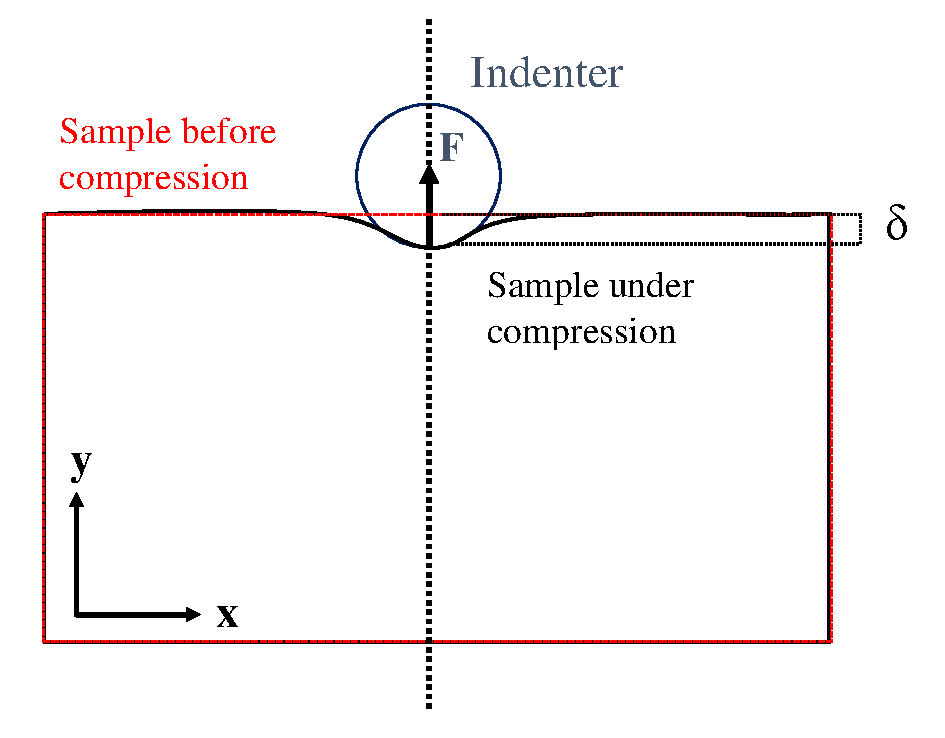
\includegraphics[width=1\linewidth]{Figures/Hertz Contact.pdf}  
    \end{subfigure}
    \hfill
    \begin{subfigure}[t]{0.45\textwidth}
        \centering
        \caption{\label{fig: Sphere-Plane_Result}}
        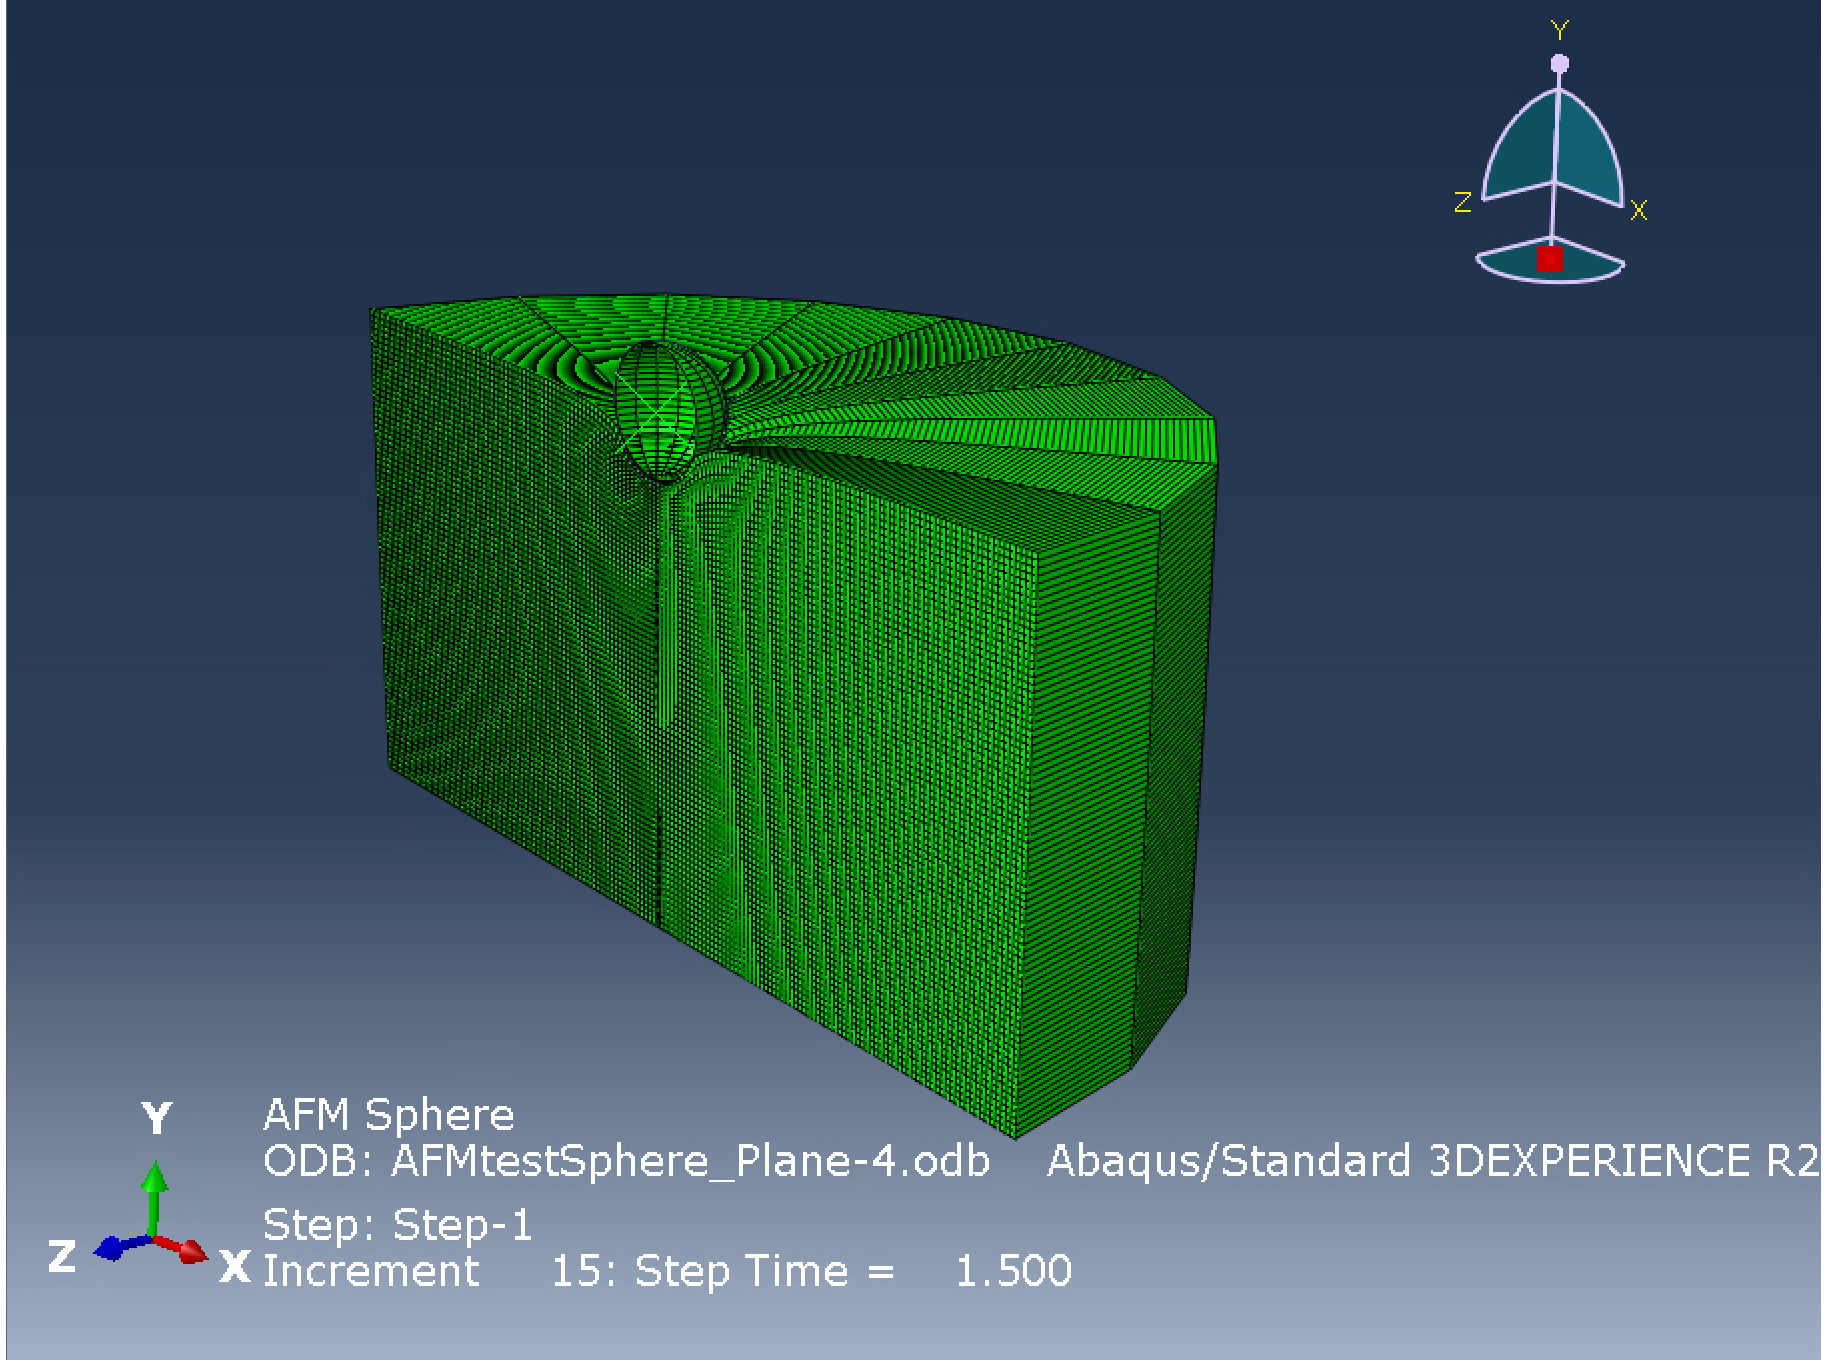
\includegraphics[width=1\linewidth]{Figures/Sphere-Plane_Result.png}        
    \end{subfigure}
    
    \hfill
    
    \begin{subfigure}[t]{0.32\textwidth}
        \centering
        \caption{\label{fig: Sphere-Plane-Force_Curve} }
        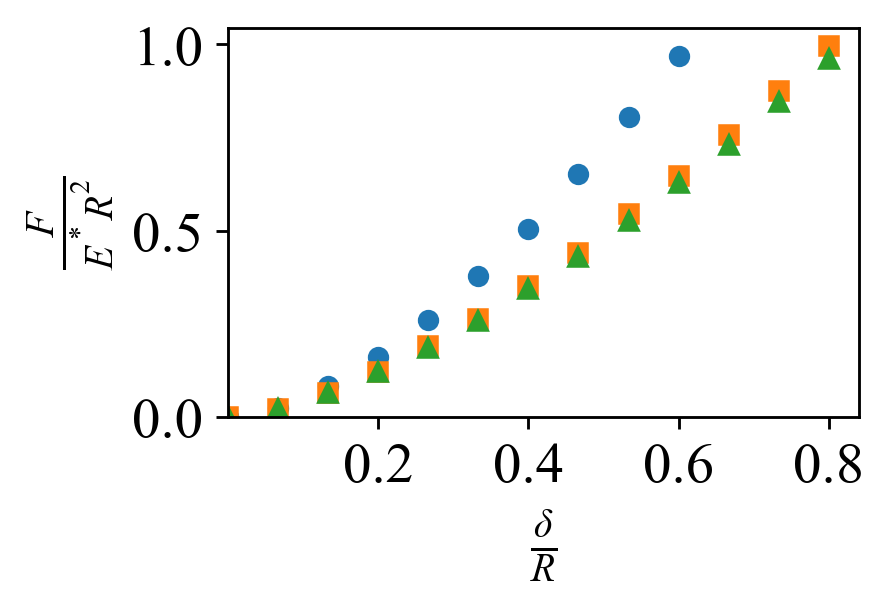
\includegraphics[width=1\linewidth]{Figures/Sphere-Plane-Force_Curve-Indenter.png}
    \end{subfigure}
    \hfill
    \begin{subfigure}[t]{0.32\textwidth}
        \centering
        \caption{\label{fig: Cone-Plane-Force_Curve} }
        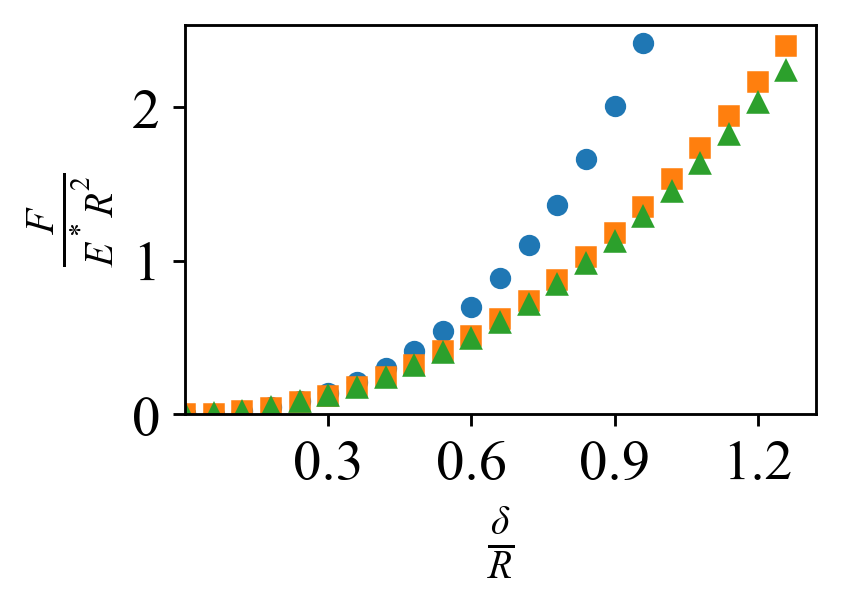
\includegraphics[width=1\linewidth]{Figures/Cone-Plane-Force_Curve-Indenter.png}
    \end{subfigure}
    \hfill
    \begin{subfigure}[t]{0.32\textwidth}
        \centering
        \caption{\label{fig: Capped-Plane-Force_Curve}}
        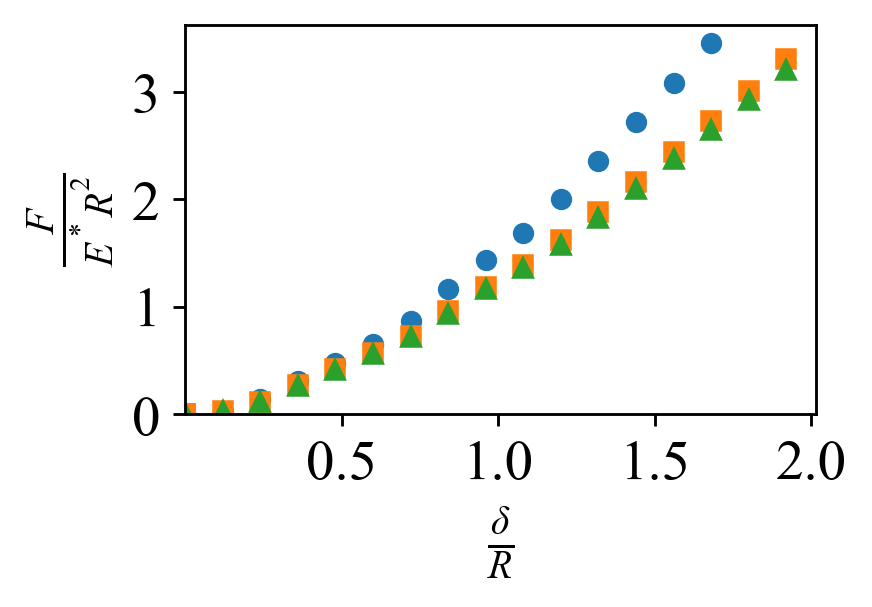
\includegraphics[width=1\linewidth]{Figures/Capped-Plane-Force_Curve-Indenter.png}
    \end{subfigure}

    \hfill
    
    \begin{subfigure}[t]{1\textwidth}
        
\includegraphics[width=1\linewidth]{Figures/Planes-Force_Curve-Legend.png}
    \end{subfigure}
    
    \caption{\label{fig: Force_Curve-Planes}(A) Illustration of contact experienced by elastic half-space for indentation depth $\delta$, and force, $F$. (B) Visualisation from  GUI for the sphere-plane indentation where the asymmetric model is rotated 180 degrees around the central axis. (C)-(E) Force curves for indentation into an elastic half-space with varying plane depth and radius, h. Given in dimensionless units of force ($\frac{F}{E^*R^2}$) and indentation ($\delta/R$). (C) Force curve for spherical indenter. (D) Force curve for conical indenter with half-angle of $\alpha = 60^o$. (E) Force curve for capped conical indenter with a half-angle of $\alpha = 20^o$. To normalise conical indenter data R is set as max contact radius $R=\delta_{max}\tan(\alpha)$. } 
    
\end{figure}

As shown in Figure \ref{fig: Force_Curve-Planes}, these simulations gave the characteristic force curves for each indenter. For greater applicability, the simulation data is analysed in dimensionless units of force and relative indentation, which are scaled using the Hertz contact equation (given in Appendix \ref{Appendix: Hertz}). The conical indenter shows the most significant curvature in its force curve. This is because contact forces are distributed more over the spherical surfaces than the sharper tip. Therefore, the conical indenter produces more prominent deformation for the same force.  

In comparison, the capped conical indenter produced a curve with transitional behaviour around $\delta/R=1$, which is expected as the indenter moves from the spherical portion to the conical. Moreover, as the surface size (h) increases, the area bounded by the curves decreases. As the area under the curve represents the elastic energy of indentation, this behaviour illustrates the increased energy required to compress smaller planes. This is because the indention on smaller surfaces causes significant horizontal shear stress, and indention to the same depth cause more extensive compression. Therefore, this effectively produces greater stiffness and elastic energy. 

\begin{figure}[H]
\centering

    \begin{subfigure}[t]{0.32\textwidth}
        \centering
        \caption{\label{fig: Sphere-Plane-Setup}}
        \includegraphics[width=1\linewidth]{Figures/Sphere-Plane-Setup.png}
    \end{subfigure}  
    \hfill
    \begin{subfigure}[t]{0.32\textwidth}
        \centering
        \caption{\label{fig: Sphere-Plane-Contact_Models}  }
        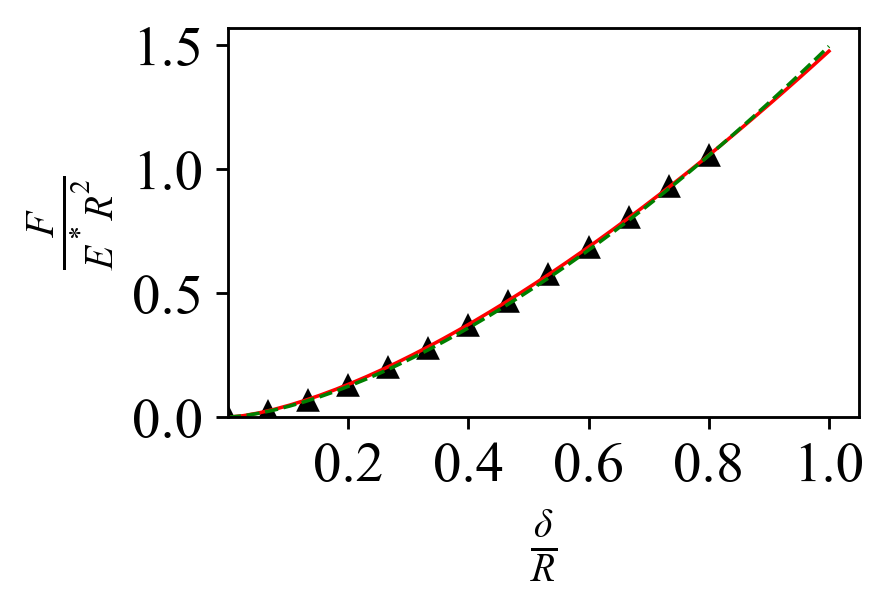
\includegraphics[width=1\linewidth]{Figures/Sphere-Plane-Contact_Models.png}
    \end{subfigure}
    \hfill
   \begin{subfigure}[t]{0.32\textwidth}
        \centering
        \caption{\label{fig: Sphere-Plane-Young's_Modulus} }
        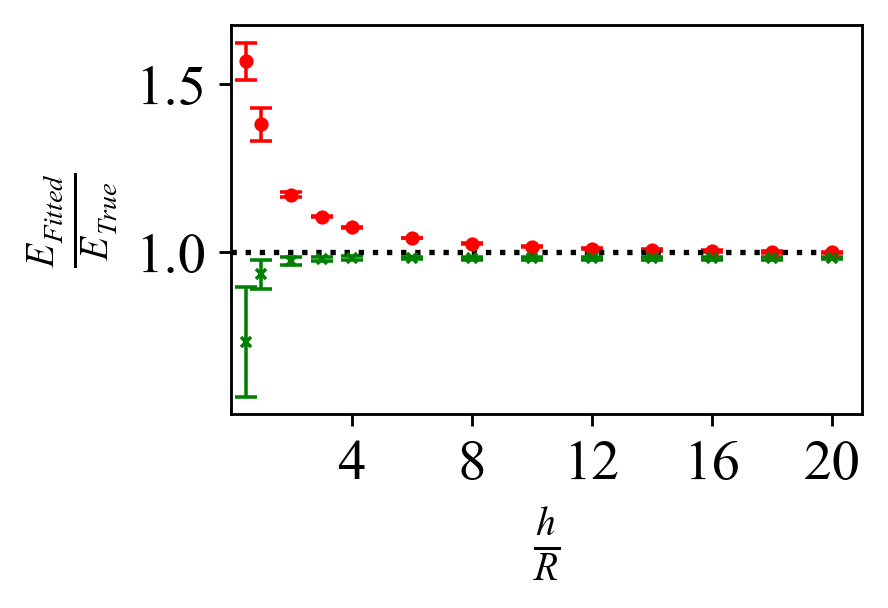
\includegraphics[width=1\linewidth]{Figures/Sphere-Plane-Youngs_Modulus.png}
    \end{subfigure} 

    
    \hfill
    \vspace{-0.4in}
    
    \begin{subfigure}[t]{0.32\textwidth}
        \centering
        \caption{\label{fig: Capped-Plane-Setup}}
        \includegraphics[width=1\linewidth]{Figures/Capped-Plane-Setup.png}
    \end{subfigure}
    \hfill
    \begin{subfigure}[t]{0.32\textwidth}
        \centering
        \caption{\label{fig: Capped-Plane-Contact_Models}  }
        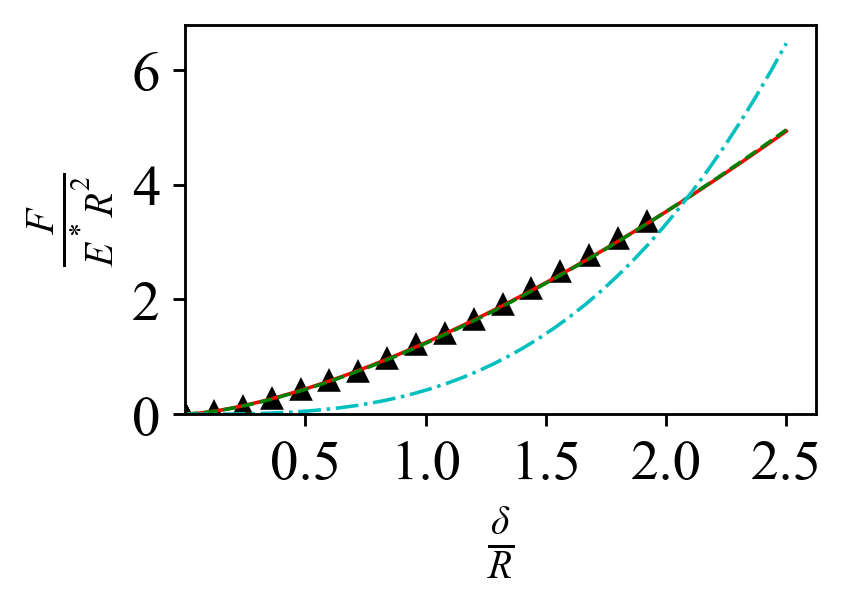
\includegraphics[width=1\linewidth]{Figures/Capped-Plane-Contact_Models.png}
    \end{subfigure}
    \hfill
    \begin{subfigure}[t]{0.32\textwidth}
        \centering
        \caption{\label{fig: Capped-Plane-Young's_Modulus} }
        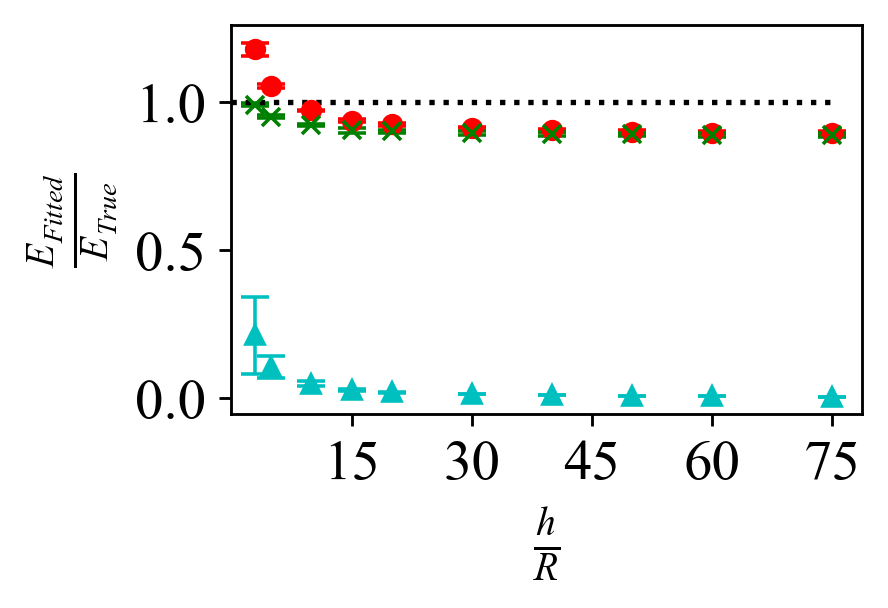
\includegraphics[width=1\linewidth]{Figures/Capped-Plane-Youngs_Modulus.png}
    \end{subfigure}

    
    \hfill
    \vspace{-0.4in}
    
    \begin{subfigure}[t]{0.32\textwidth}
        \centering
        \caption{\label{fig: Cone-Plane-Setup}}
        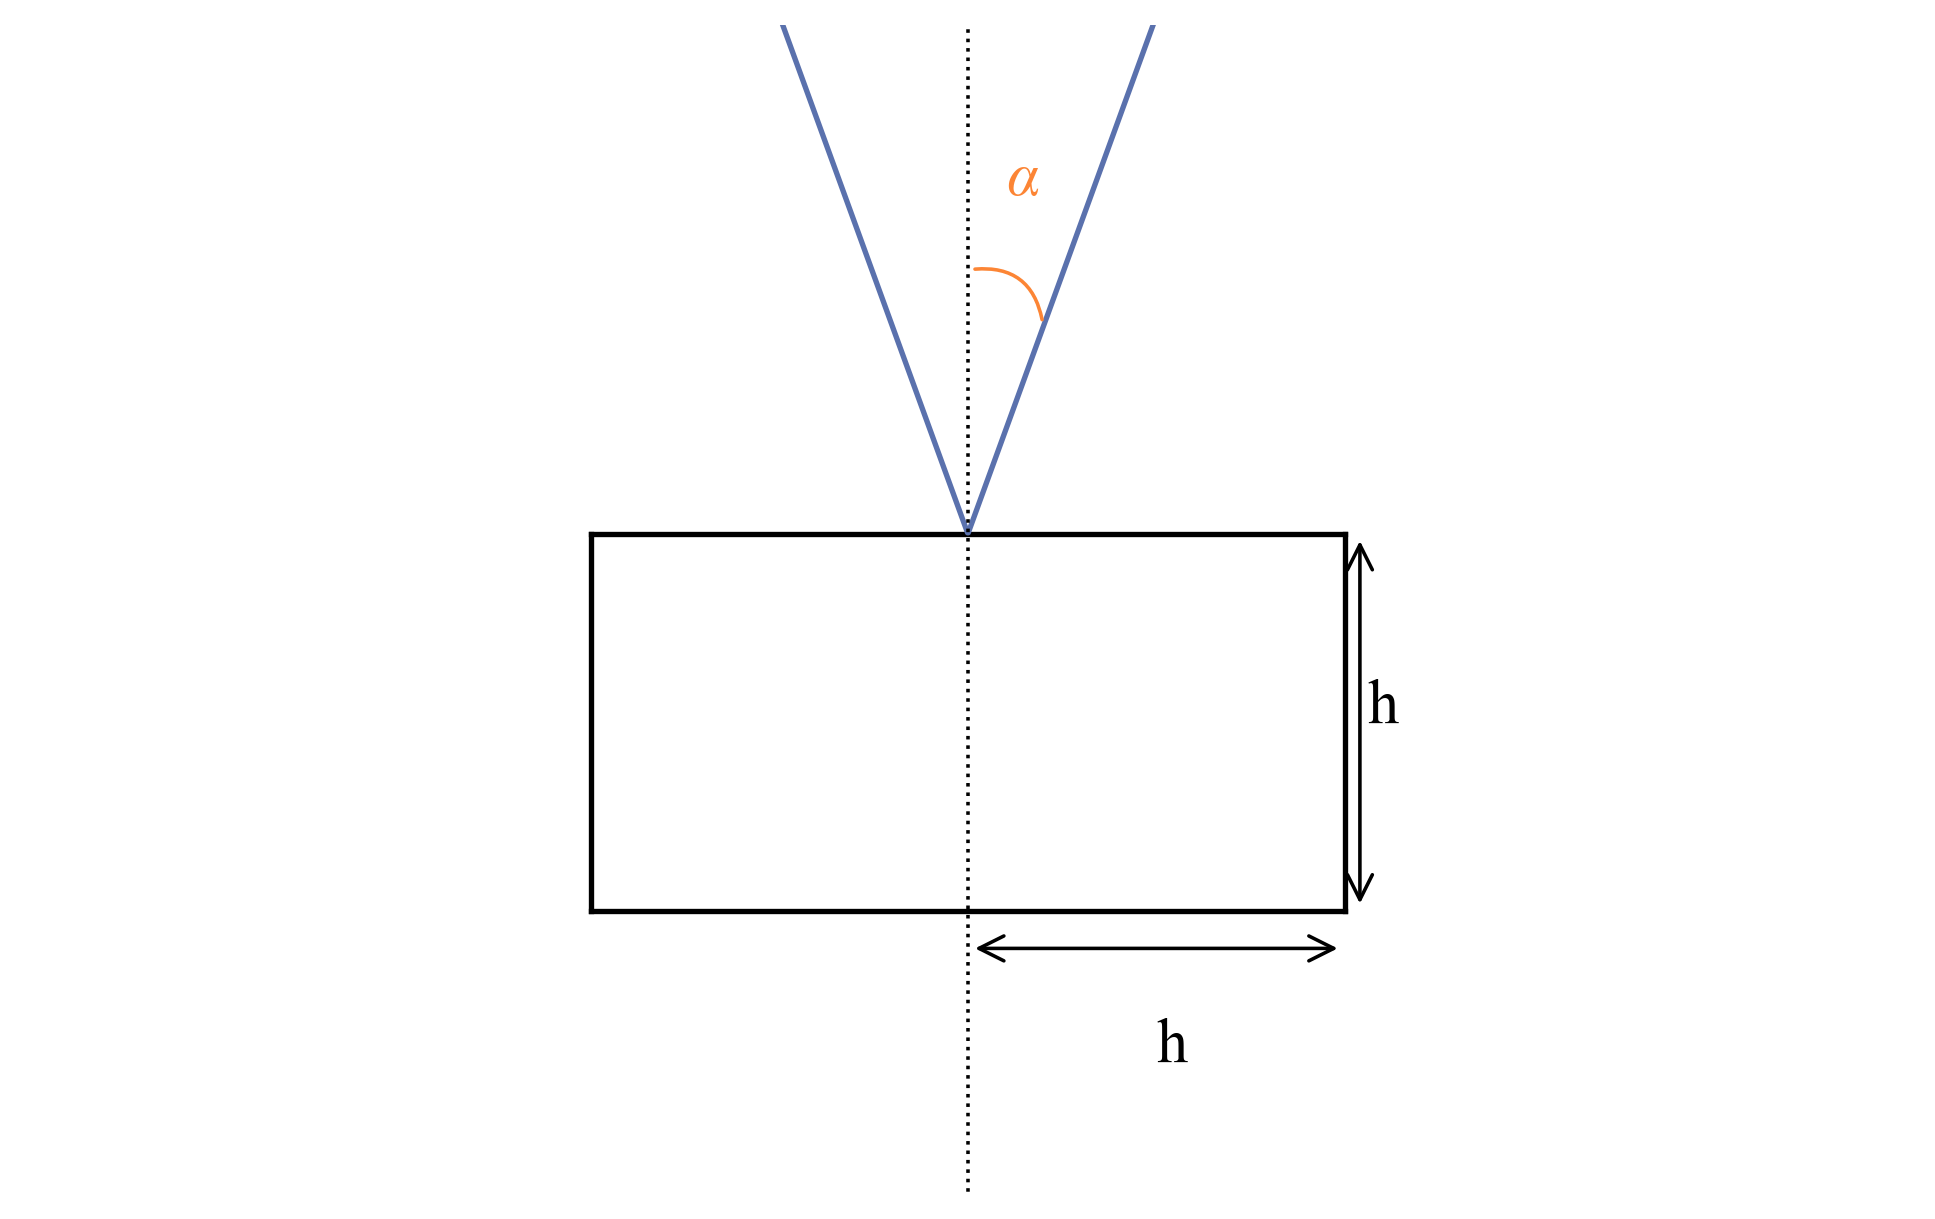
\includegraphics[width=1\linewidth]{Figures/Cone-Plane-Setup.png}
    \end{subfigure}  
    \hfill  
    \begin{subfigure}[t]{0.32\textwidth}
        \centering
        \caption{\label{fig: Cone-Plane-Contact_Models} }
        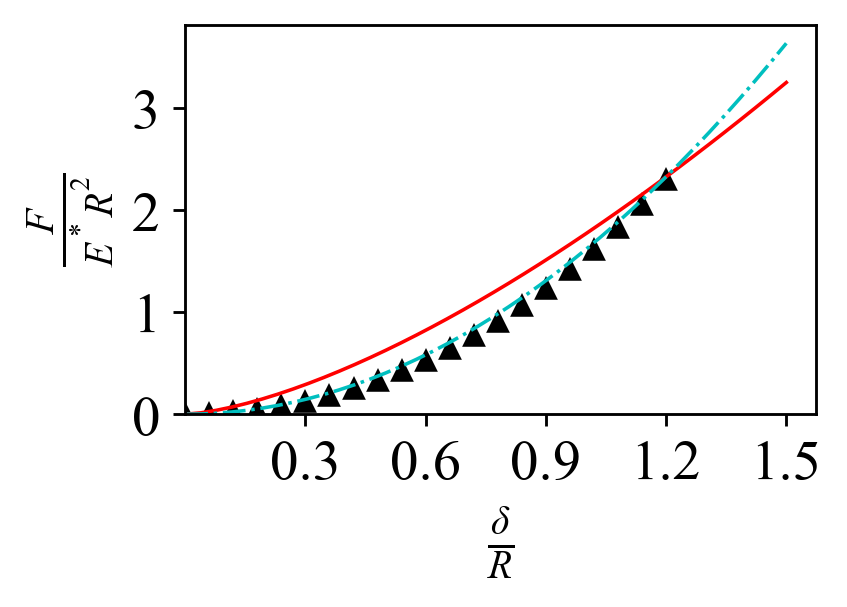
\includegraphics[width=1\linewidth]{Figures/Cone-Plane-Contact_Models.png}
    \end{subfigure}
    \hfill
    \begin{subfigure}[t]{0.32\textwidth}
        \centering
        \caption{\label{fig: Cone-Plane-Young's_Modulus} }
        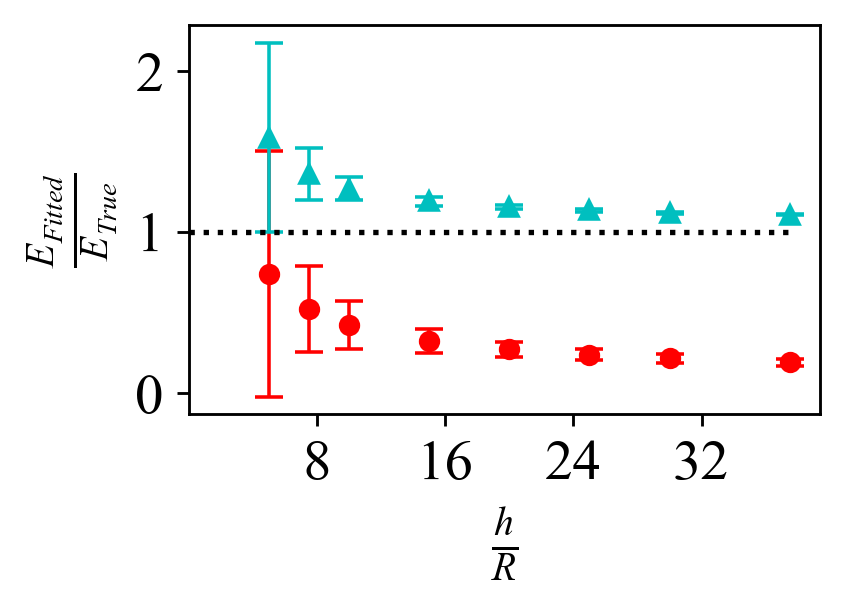
\includegraphics[width=1\linewidth]{Figures/Cone-Plane-Youngs_Modulus.png}
    \end{subfigure}
    
    \hfill
    
    \begin{subfigure}[t]{1\textwidth}
        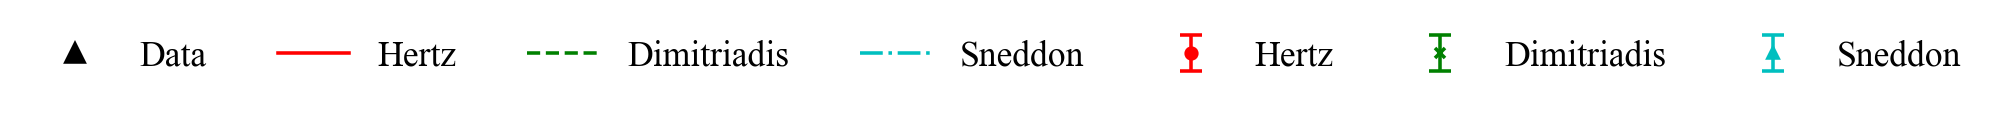
\includegraphics[width=1\linewidth]{Figures/Planes-Legend.png}
    \end{subfigure}
    
    \caption{\label{fig: Plane-Data}(A) Model assembly for spherical indentation of elastic half-space. (B) Plot for spherical indentation force curves fitted using the Hertz and Dimitriadis models. (C) Young's Modulus variation for spherical indentation into elastic half-space. (D) Model assembly for spherically-capped conical indentation of an elastic half-space. (E) Plot for capped indentation force curves fitted using the Hertz, Dimitriadis, and Sneddon models. (F) Young's Modulus variation for conical indentation into elastic half-space. (G) Model assembly for conical indentation of an elastic half-space. (H) Plot for conical indentation force curves fitted using the Hertz and Sneddon models. (I) Young's Modulus variation for conical indentation into elastic half-space. For conical indenter data normalisation $R=\delta_{max}\tan(\alpha)$.}  
    
\end{figure}

Fitting the contact models to the simulated data for the spherical indenter, shown in Figure \ref{fig: Sphere-Plane-Contact_Models}, showed good adherence from both Hertz and Dimitriadis models. Moreover, comparing the fitted Young's modulus for increasing surface geometry, in Figure \ref{fig: Sphere-Plane-Young's_Modulus}, shows both models converged on the expected Young's modulus, confirming the accuracy of the simulation dynamics. However, there was a significant divergence from the predicted Young's modulus at small surface geometry and a greater error in the fit. This behaviour is expected as the indenter is a comparable size to the surface at smaller surface dimensions. Therefore, the force is distributed over a larger portion of the surface and can cause buckling and shear forces as the plane bulges out. In addition, this can create larger reaction forces at the base. Consequently, this creates deviation from the theoretical models along with the contradiction of the assumption of an elastic half-space with an infinite horizontal/vertical extent.

Similarly, for the capped conical indenter, the Hertz and Dimitriadis model provided a much tighter fit to the data than the Sneddon model, which deviated as shown in Figure \ref{fig: Capped-Plane-Contact_Models}. This indicates that the spherical behaviour dominates over the conical behaviour at these ranges. This qualitative behaviour is further reinforced by the variation of Young's modulus over surface depth/radius shown in Figure \ref{fig: Capped-Plane-Young's_Modulus}. The Sneddon model converges on zero, indicating that the model diverges to a large extent and is a poor description of the indentation. In contrast, the Hertz and Dimitriadis models converged closely on the expected Young's modulus. Some deviation is expected as the models are for a pure spherical indenter, whereas the conical section of the capped indenter causes variation in the contact. 

Lastly, the Sneddon model produced an expected tight fit for the conical indenter, whereas Hertz was a poor fit. As expected, the Hertz model failed to converge upon the correct Young's Modulus and produced a large underfit because the model is for smaller spherical deformation. However, the Sneddon model converges to the true value. These results all provided the expected behaviours and confirmed the accuracy of ABAQUS. This provides the basis to be applied to simulations of AFM imaging.